% article example for classicthesis.sty
\documentclass[10pt,a4paper]{article} % KOMA-Script article scrartcl
\usepackage{lipsum}
\usepackage{subfigure}
\usepackage{braket}
\usepackage[utf8]{inputenc}
\usepackage{amsmath}
\usepackage{url}
\usepackage[nochapters]{classicthesis} % nochapters
\usepackage{listings}
\usepackage[pdftex]{graphicx}
\renewcommand{\i}{{\mathrm{i}}}
\renewcommand{\d}{\mathrm{d}}
\begin{document}
    \title{\rmfamily\normalfont\spacedallcaps{Quantum Many-Body Simulations in Haskell}}
    \author{\spacedlowsmallcaps{David Schlegel}}
    \date{01.10.15} % no date
    	
    
    \maketitle
    
    \begin{abstract}
      Applying numerical methods in quantum mechanics has always been necessary in analysing complex structures of quantum mechanical systems. The technical progress of computer performance has enabled physicists and mathematicians to simulate complex many-body systems. With these methods tangible progress in quantum physics can be made, to analyse quantum phenomena on the level of many-particle interactions. This article focuses on the implementation of numerical methods for many-body simulation in the functional programming language \textbf{Haskell}. Functional programming languages get more and more interesting for physicists through their mathematical way of implementation. In this article simple quantum systems are simulated first and an overview of different numerical methods for solving the Schrödinger equation will be given following an attempt to proceed to many-body systems from simple quantum systems. 
    \end{abstract}
       
    \tableofcontents
    
    \section{Simple Quantum Systems}\label{1}
   In this chapter simple quantum systems will be studied. Consider a particle in a three-dimensional potential $V(\vec{x})$. The corresponding wave function $\psi(\vec{x}, t)$ is the solution of the Schrödinger equation
   \begin{equation}
  \i \hbar \frac{\partial}{\partial t} \psi(\vec{x}, t) = H \psi(\vec{x}, t) = - \frac{\hbar^2}{2m}	\Delta \psi(\vec{x}, t)+  V(\vec{x}) \psi(\vec{x}, t) \text{,}
   \end{equation}
   where $\Delta$ is the Laplacian differential operator: $\Delta = \frac{\partial^2}{\partial x^2} +\frac{\partial^2}{\partial y^2} + \frac{\partial^2}{\partial z^2} $. For a time-independent potential $V(\vec{x})$ the Schrödinger equation can be formally solved by 
   
   \begin{equation}
     \psi(\vec{x}, t) = \text{U}(t, t_0) \psi(\vec{x}, t_0)   = \exp \left\{ - \frac{\i (t-t_0) }{\hbar} H \right\}  \psi(\vec{x}, t_0) \text{.}
   \end{equation} 
   For a time-dependent potential like an oscillating laserfield, the time evolution of the wave function becomes
   \begin{align}
   \psi(\vec{x}, t) &= \text{U}(t, t_0) \psi(\vec{x}, t_0)  = \hat{\text{T}}_t  \exp \left\{ \frac{\i}{h} \int_{t_0}^t H(\tau) \d \tau \right \}  \psi(\vec{x}, t_0)  \\
   &=  \sum_{n = 0}^\infty \frac{1}{n} {\left( \frac{- \i}{\hbar} \right) }^n \int_{t_0}^t \d t_1\int_{t_0}^t \d t_2 \dots \int_{t_0}^t \d t_n \hat{\text{T}}_t \left\{ H(t_1)H(t_2) \dots H(t_n) \right\} \text{,} \nonumber
   \end{align} 
   where $\hat{\text{T}}_t$ is the time ordering operator. A simple approach is to divide the interval $[0 \dots t]$ into a sequence of $N$ steps so that
   \begin{equation}
   \text{U}(t, t_0) = \text{U}(t, t_{N-1}) \dots \text{U}(t_2, t_1)\text{U}(t_1, t_0)
\end{equation}   and to neglect small deviations of the Hamiltonian in the small interval $\Delta t = t_n - t_{n-1}$.
   
    \subsection{Discretization of the kinetic Energy}
    Dividing the Hamiltonian $H$ into $H = T + V$, the non-local kinetic energy operator can be written as
    \begin{equation}
    T \psi(\vec{x}, t) = - \frac{\hbar^2}{2m} \Delta \psi(\vec{x}, t) \text{.}
    \end{equation}
    
    \subsubsection{Method of Finite Differences}
    Taking a grid $(k,l,m)$ in three dimensions, the kinetic energy operator can be approximated by finite differences
    \begin{flalign}
   &  T \psi(\vec{x}, t) =  - \frac{\hbar^2}{2m}  \left(  
     \frac{\psi_{(k+1,l,m)}^n -2 \psi_{(k,l,m)}^n + \psi_{(k-1,l,m)}^n}{\Delta x^2} +\right. \nonumber \\
     & \left . \frac{\psi_{(k,l+1,m)}^n -2 \psi_{(k,l,m)}^n + \psi_{(k,l-1,m)}^n}{\Delta y^2} +
       \frac{\psi_{(k,l,m+1)}^n -2 \psi_{(k,l,m)}^n + \psi_{(k,l,m-1)}^n}{\Delta z^2} \right)
    \end{flalign} with higher order terms $\mathcal{O}(\Delta x^2, \Delta y^2, \Delta z^2 )$ where $n$ represents the discrete time index of the wave function. Considering the time independent Schrödinger equation we can write the operator in one dimension as a matrix satisfying the eigenvalue equation
 \begin{align}
\left[ \begin{pmatrix}
2	& -1	& &  \dots	 & 0      \\
-1	& 2 	&  -1&  & \vdots	  \\
\vdots	& \ddots 	& \ddots &  \ddots & \\
&  &-1 & 2 & -1\\
0 	&   \dots & & -1	 & 2
\end{pmatrix} + V_{kk} \right ]
\begin{pmatrix}\psi_1 \\ \vdots \\ \psi_k \\ \vdots \\ \psi_N \end{pmatrix}
 = E \begin{pmatrix}\psi_1 \\ \vdots \\ \psi_k \\ \vdots \\ \psi_N \end{pmatrix}
\end{align} where $\vec{\psi}$ are the values of the wave function on the evaluation points $x_k$. $V_{kk}$  represents the potential for each $x_k$, thus it is a diagonal matrix.
\par For the example of a particle in a box the potential is
\begin{align} 
V_{kk} = \left\{ \begin{array}{ll}  \infty  \quad \text{for} \quad  k = 0, \; k= N \\  0 \quad \text{else} \end{array} \right. \text.
\end{align}
Solving the above eigenvalue equation yields the eigenfunctions $\psi_n$ with eigenenergies $E_n$. The boundary conditions $V = \infty$ at $k=0$ and $k=N$ are satisfied even when the boundary conditions are left out. An example of the first four eigenstates is shown in \mbox{ figure \ref{fig:eigenfunctions}.}
\begin{figure}[!htb]
	\Huge
	\centering
	\resizebox{!}{0.6\textwidth}{%% Creator: Inkscape inkscape 0.91, www.inkscape.org
%% PDF/EPS/PS + LaTeX output extension by Johan Engelen, 2010
%% Accompanies image file 'eigenfunctions.pdf' (pdf, eps, ps)
%%
%% To include the image in your LaTeX document, write
%%   \input{<filename>.pdf_tex}
%%  instead of
%%   \includegraphics{<filename>.pdf}
%% To scale the image, write
%%   \def\svgwidth{<desired width>}
%%   \input{<filename>.pdf_tex}
%%  instead of
%%   \includegraphics[width=<desired width>]{<filename>.pdf}
%%
%% Images with a different path to the parent latex file can
%% be accessed with the `import' package (which may need to be
%% installed) using
%%   \usepackage{import}
%% in the preamble, and then including the image with
%%   \import{<path to file>}{<filename>.pdf_tex}
%% Alternatively, one can specify
%%   \graphicspath{{<path to file>/}}
%% 
%% For more information, please see info/svg-inkscape on CTAN:
%%   http://tug.ctan.org/tex-archive/info/svg-inkscape
%%
\begingroup%
  \makeatletter%
  \providecommand\color[2][]{%
    \errmessage{(Inkscape) Color is used for the text in Inkscape, but the package 'color.sty' is not loaded}%
    \renewcommand\color[2][]{}%
  }%
  \providecommand\transparent[1]{%
    \errmessage{(Inkscape) Transparency is used (non-zero) for the text in Inkscape, but the package 'transparent.sty' is not loaded}%
    \renewcommand\transparent[1]{}%
  }%
  \providecommand\rotatebox[2]{#2}%
  \ifx\svgwidth\undefined%
    \setlength{\unitlength}{800bp}%
    \ifx\svgscale\undefined%
      \relax%
    \else%
      \setlength{\unitlength}{\unitlength * \real{\svgscale}}%
    \fi%
  \else%
    \setlength{\unitlength}{\svgwidth}%
  \fi%
  \global\let\svgwidth\undefined%
  \global\let\svgscale\undefined%
  \makeatother%
  \begin{picture}(1,0.75)%
    \put(0,0){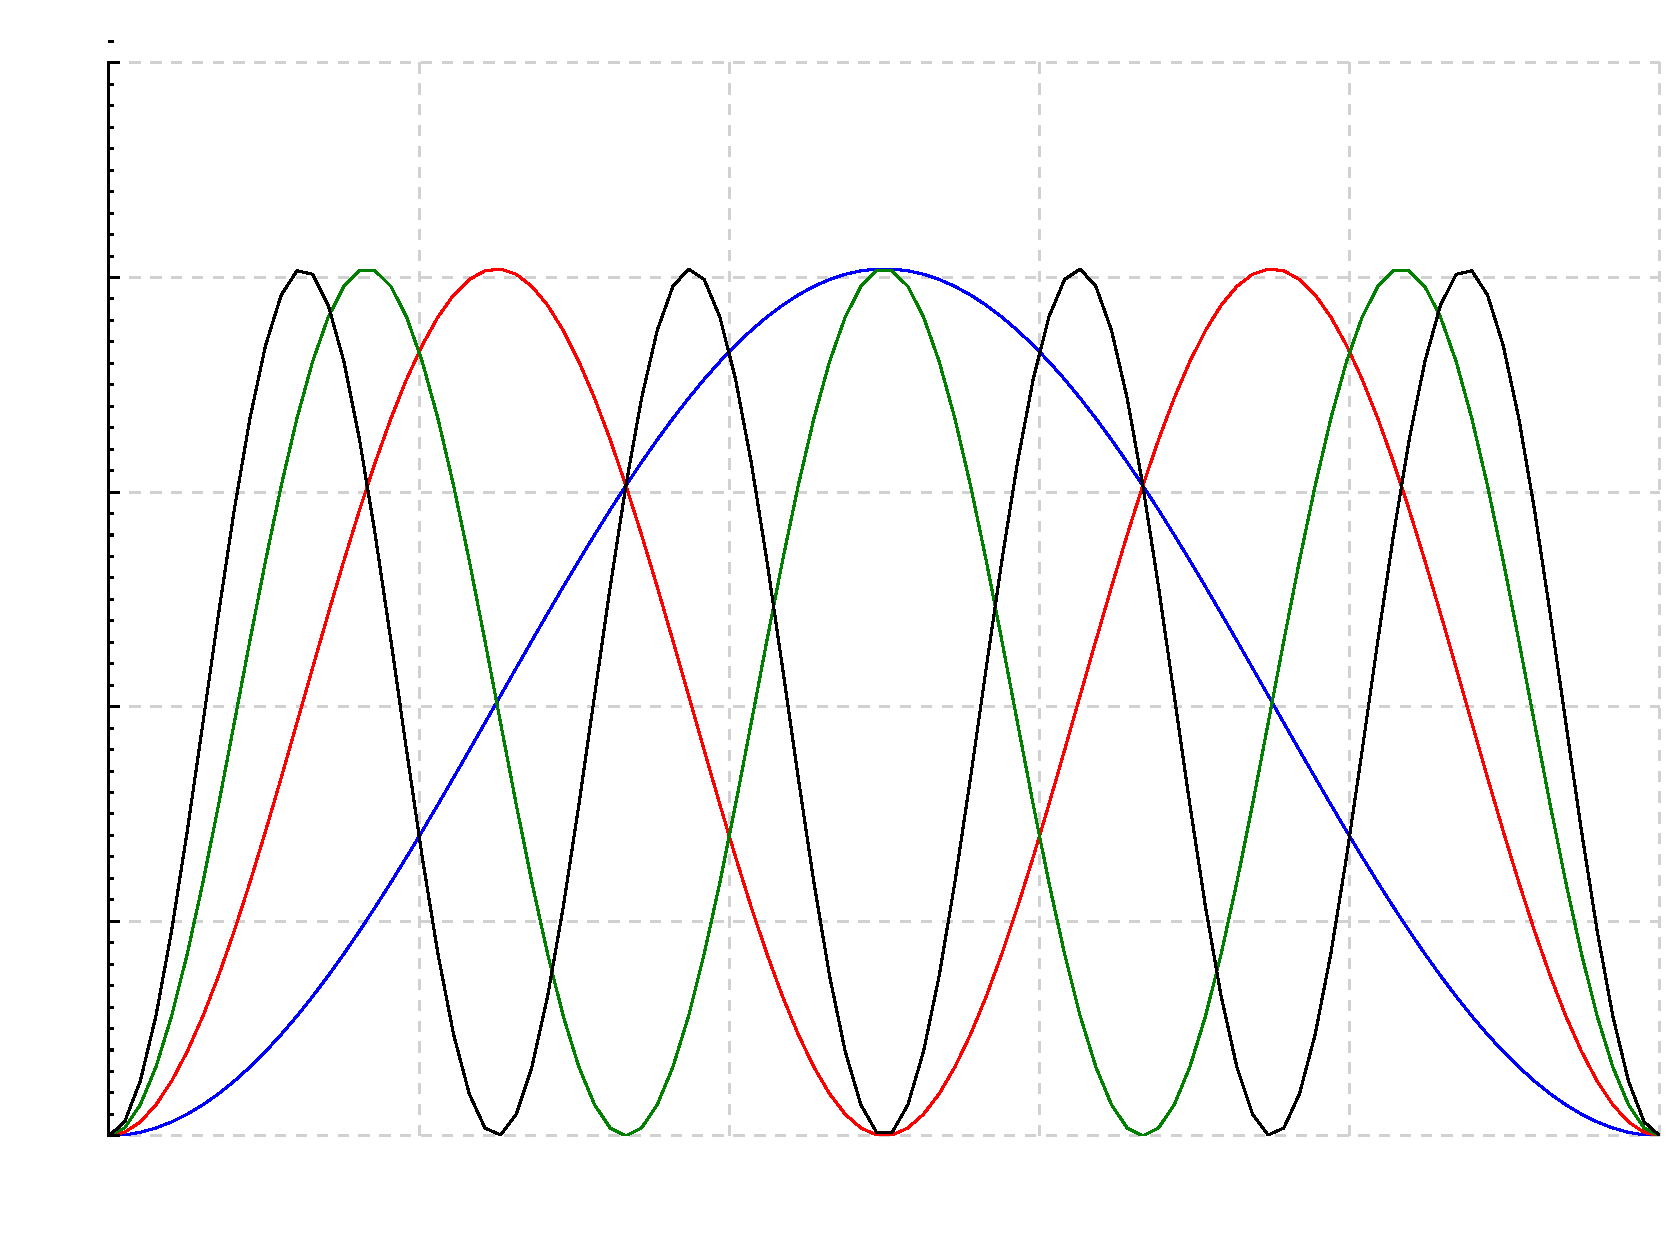
\includegraphics[width=\unitlength,page=1]{figures/eigenfunctions.pdf}}%
    \put(0.004,0.57681454){\color[rgb]{0,0,0}\makebox(0,0)[lb]{\smash{$0.02$}}}%
    \put(0,0){\includegraphics[width=\unitlength,page=2]{figures/eigenfunctions.pdf}}%
    \put(0.0,0.44990405){\color[rgb]{0,0,0}\makebox(0,0)[lb]{\smash{$0.015$}}}%
    \put(0.004,0.32290405){\color[rgb]{0,0,0}\makebox(0,0)[lb]{\smash{$0.01$}}}%
    \put(0.0,0.70690405){\color[rgb]{0,0,0}\makebox(0,0)[lb]{\smash{$0.025$}}}%
    \put(0.004,0.06340405){\color[rgb]{0,0,0}\makebox(0,0)[lb]{\smash{$0$}}}%
    \put(0.004,0.19197949){\color[rgb]{0,0,0}\makebox(0,0)[lb]{\smash{$0.05$}}}%
    \put(0.03773901,0.04840405){\color[rgb]{0,0,0}\makebox(0,0)[lb]{\smash{$0$}}}%
    \put(0.23223901,0.04){\color[rgb]{0,0,0}\makebox(0,0)[lb]{\smash{$0.2$}}}%
    \put(0.41073901,0.03){\color[rgb]{0,0,0}\makebox(0,0)[lb]{\smash{$0.4$}}}%
    \put(0.59823901,0.03){\color[rgb]{0,0,0}\makebox(0,0)[lb]{\smash{$0.6$}}}%
    \put(0.783239,0.03){\color[rgb]{0,0,0}\makebox(0,0)[lb]{\smash{$0.8$}}}%
    \put(0.970739,0.03){\color[rgb]{0,0,0}\makebox(0,0)[lb]{\smash{$1$}}}%
    \put(0.04823902,0.02040406){\color[rgb]{0,0,0}\makebox(0,0)[lb]{\smash{$\psi_1$}}}%
    \put(0.13614134,0.0200705){\color[rgb]{0,0,0}\makebox(0,0)[lb]{\smash{$\psi_2$}}}%
    \put(0.21064144,0.02057045){\color[rgb]{0,0,0}\makebox(0,0)[lb]{\smash{$\psi_3$}}}%
    \put(0.29614145,0.01957047){\color[rgb]{0,0,0}\makebox(0,0)[lb]{\smash{$\psi_4$}}}%
    \put(0.4752763,0.73714841){\color[rgb]{0,0,0}\makebox(0,0)[lb]{\smash{Eigenfunctions}}}%
  \end{picture}%
\endgroup%
}
	\caption{Propability densities for the calculated eigenfunctions $\psi_n$, with the method of finite differences and a grid of $N=100$ for $n = 1,2,3$ and $4$ in one dimension. For simplicity the pre-factor $\frac{\hbar^2}{2m}$ was set to one, obtaining non-normalized eigenfunctions.}
	\label{fig:eigenfunctions}
\end{figure} 
To reduce the problem of a particle in three dimensions to a simple matrix equation, the spatial wave function $\vec{\psi}$ can be stacked, to obtain an $N^3$ dimensional vector
\begin{align}
\vec{\psi}_{k,l,m} = \begin{pmatrix}\vec{\psi}_{1,1,m} \\ \vdots \\ \vec{\psi}_{1,N,m} \\ \vdots \\ \vec{\psi}_{N,1,m} \\ \vdots \\ \vec{\psi}_{N,N,m} \end{pmatrix} \text{, through nested vectors.}
\end{align}

For two dimensions the approximated kinetic energy operator $T$ thus becomes the tridiagonal block matrix
\begin{align}
T \approx  \begin{pmatrix}
4	& -1	&  &  -1	 &     &     &  \scalebox{3}{$0$}  \\
    & \ddots	&     & 		&   \ddots   & 	& \\
    & -1 & 4 &  &  &-1 \\
-1 &      &          & 4     & -1       & & \ddots \\
    & \ddots &     &&    \ddots   &       &  \\
  \scalebox{3}{$0$}   &      & -1       &&         & -1     & 4 \\ 
\end{pmatrix} \text{.}
\end{align}

In figure \ref{fig:2d_eigenfunction} an example of an eigenstate for a particle in a two dimensional box is shown.

\begin{figure}[!htb]
	\Huge
	\hspace*{-1.5in}
	\centering
	\subfigure[Color map, $\psi_{12}$, $N=60$.]
		{\resizebox{!}{0.38\textwidth}{%% Creator: Inkscape inkscape 0.91, www.inkscape.org
%% PDF/EPS/PS + LaTeX output extension by Johan Engelen, 2010
%% Accompanies image file '2dn12.pdf' (pdf, eps, ps)
%%
%% To include the image in your LaTeX document, write
%%   \input{<filename>.pdf_tex}
%%  instead of
%%   \includegraphics{<filename>.pdf}
%% To scale the image, write
%%   \def\svgwidth{<desired width>}
%%   \input{<filename>.pdf_tex}
%%  instead of
%%   \includegraphics[width=<desired width>]{<filename>.pdf}
%%
%% Images with a different path to the parent latex file can
%% be accessed with the `import' package (which may need to be
%% installed) using
%%   \usepackage{import}
%% in the preamble, and then including the image with
%%   \import{<path to file>}{<filename>.pdf_tex}
%% Alternatively, one can specify
%%   \graphicspath{{<path to file>/}}
%% 
%% For more information, please see info/svg-inkscape on CTAN:
%%   http://tug.ctan.org/tex-archive/info/svg-inkscape
%%
\begingroup%
  \makeatletter%
  \providecommand\color[2][]{%
    \errmessage{(Inkscape) Color is used for the text in Inkscape, but the package 'color.sty' is not loaded}%
    \renewcommand\color[2][]{}%
  }%
  \providecommand\transparent[1]{%
    \errmessage{(Inkscape) Transparency is used (non-zero) for the text in Inkscape, but the package 'transparent.sty' is not loaded}%
    \renewcommand\transparent[1]{}%
  }%
  \providecommand\rotatebox[2]{#2}%
  \ifx\svgwidth\undefined%
    \setlength{\unitlength}{1669bp}%
    \ifx\svgscale\undefined%
      \relax%
    \else%
      \setlength{\unitlength}{\unitlength * \real{\svgscale}}%
    \fi%
  \else%
    \setlength{\unitlength}{\svgwidth}%
  \fi%
  \global\let\svgwidth\undefined%
  \global\let\svgscale\undefined%
  \makeatother%
  \begin{picture}(1,0.55062912)%
    \put(0,0){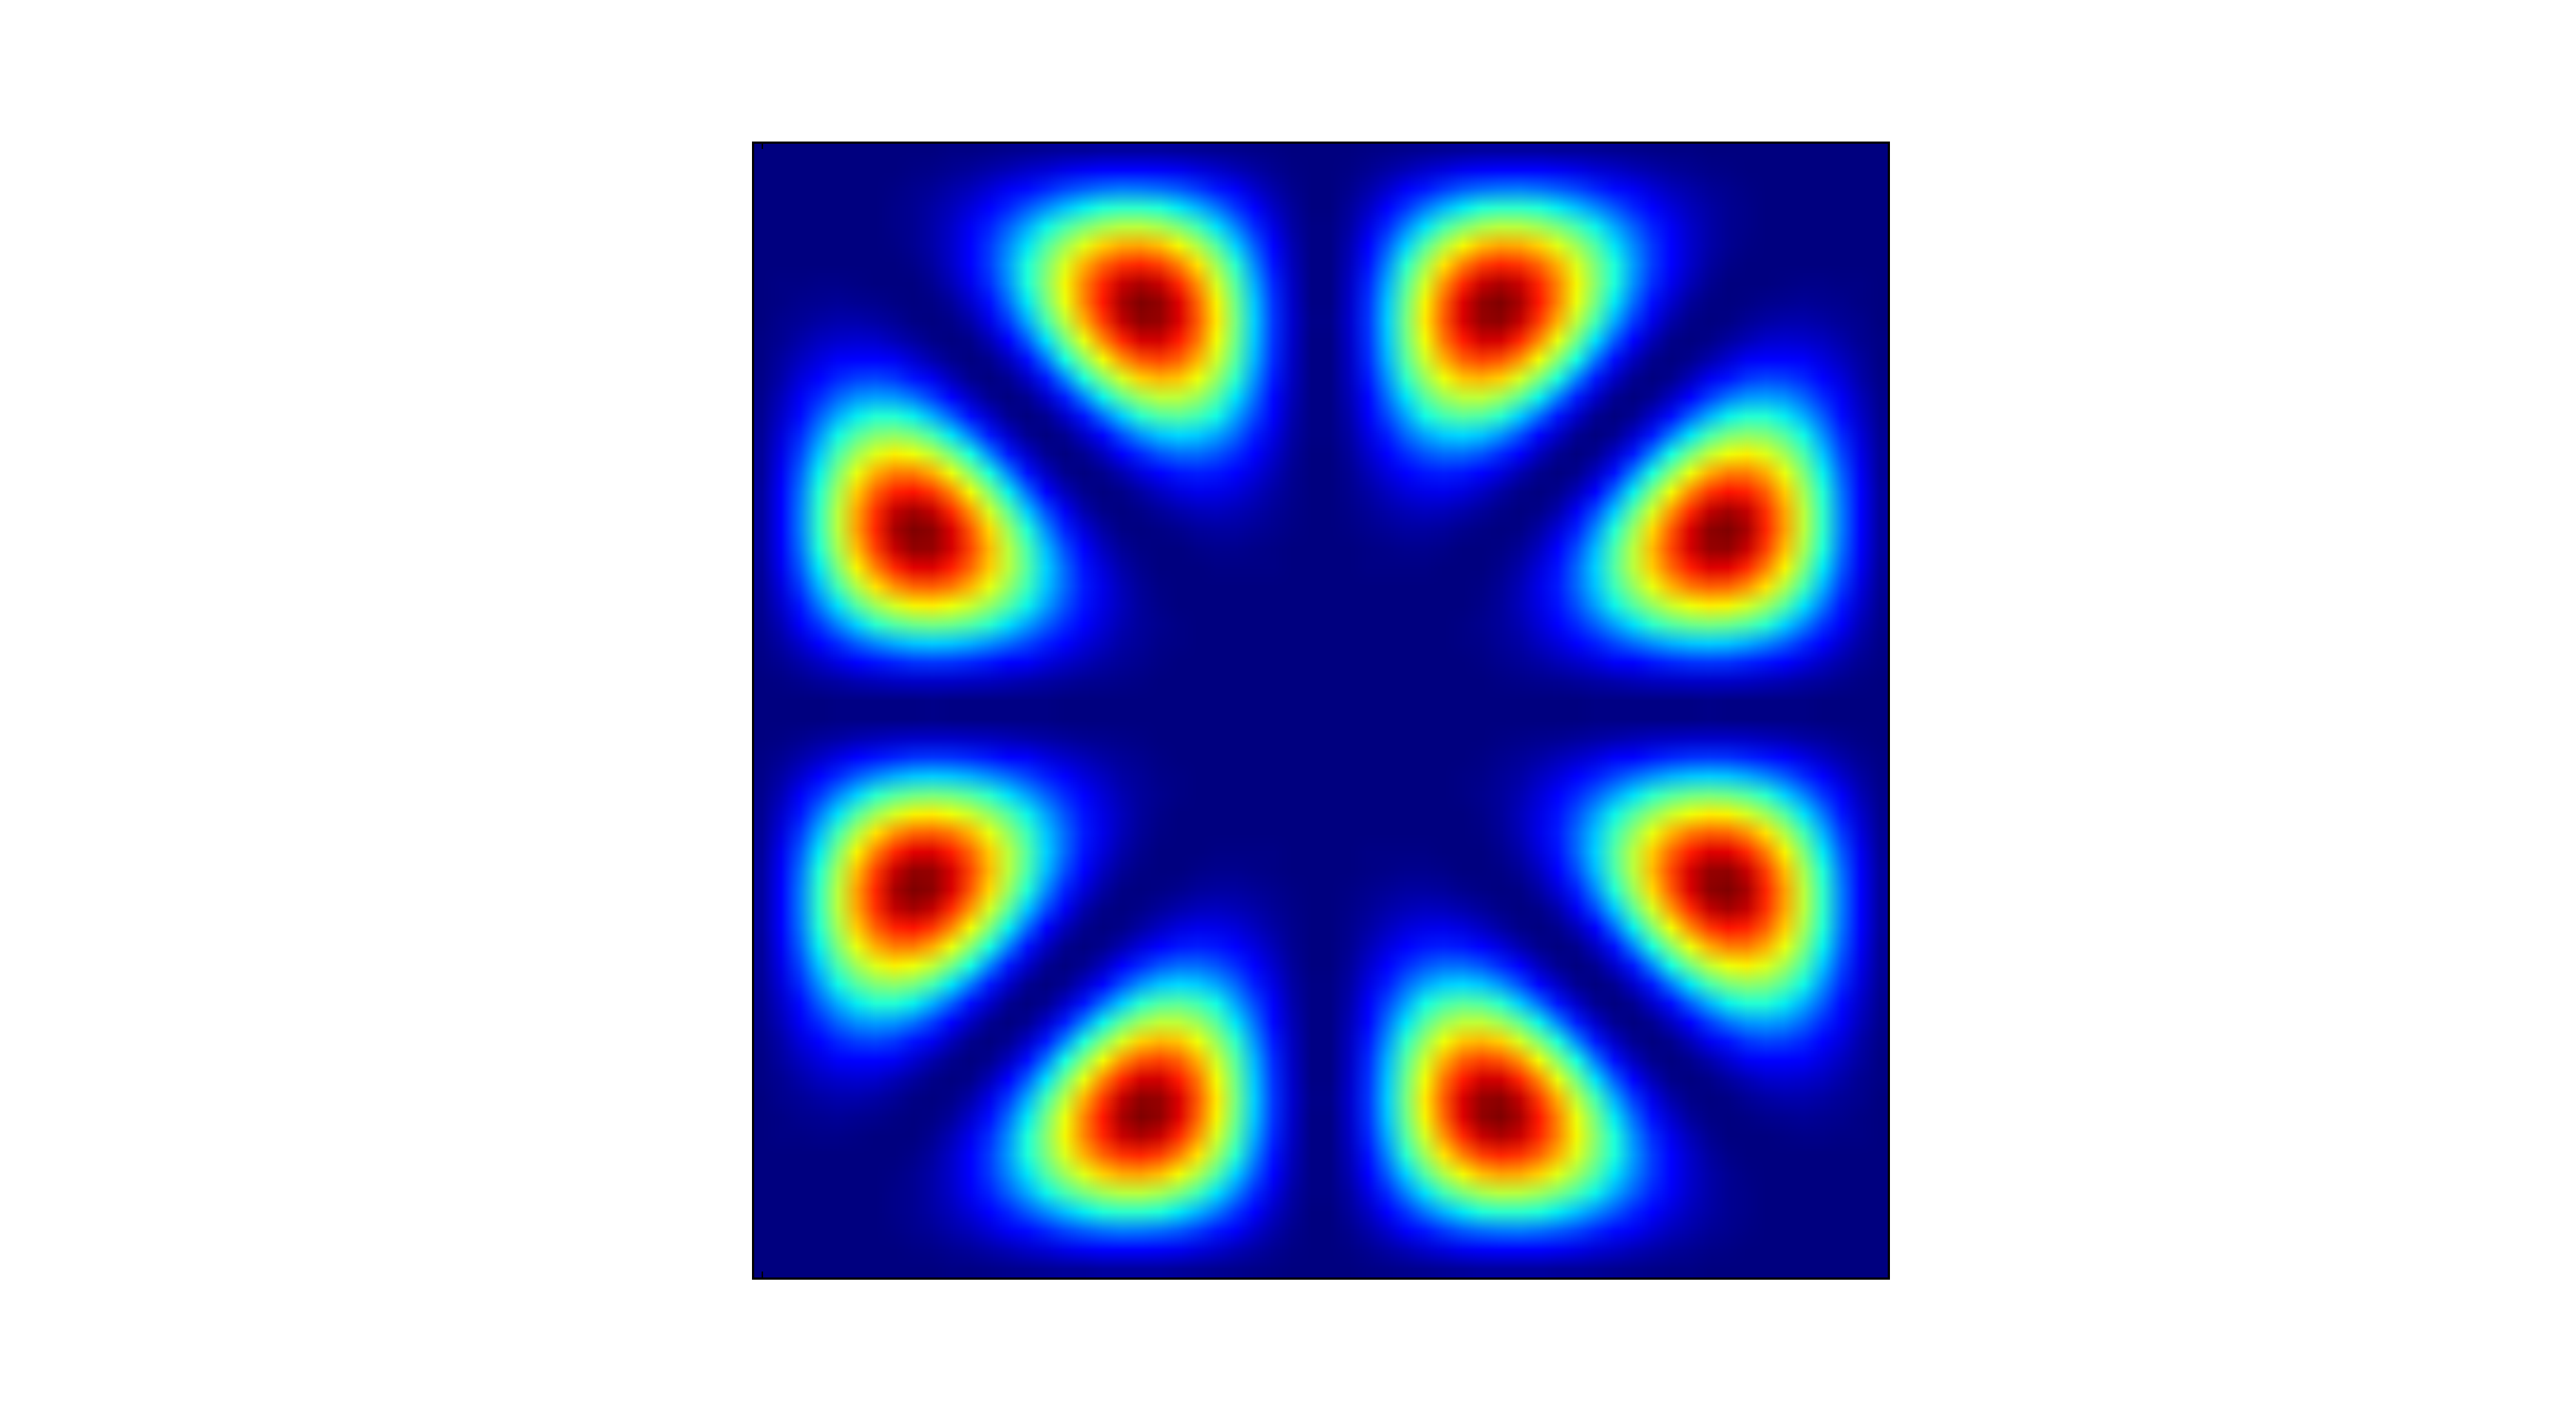
\includegraphics[width=\unitlength,page=1]{figures/2dn12.pdf}}%
    \put(0.29029359,0.02){\color[rgb]{0,0,0}\makebox(0,0)[lb]{\smash{$0$}}}%
    \put(0,0){\includegraphics[width=\unitlength,page=2]{figures/2dn12.pdf}}%
    \put(0.36680651,0.02){\color[rgb]{0,0,0}\makebox(0,0)[lb]{\smash{$0.17$}}}%
    \put(0.4426603,0.02){\color[rgb]{0,0,0}\makebox(0,0)[lb]{\smash{$0.33$}}}%
    \put(0.48651887,0.0524266){\color[rgb]{0,0,0}\makebox(0,0)[lb]{\smash{}}}%
    \put(0.51581787,0.02){\color[rgb]{0,0,0}\makebox(0,0)[lb]{\smash{$0.5$}}}%
    \put(0.58897543,0.02){\color[rgb]{0,0,0}\makebox(0,0)[lb]{\smash{$0.67$}}}%
    \put(0.66133219,0.02){\color[rgb]{0,0,0}\makebox(0,0)[lb]{\smash{$0.83$}}}%
    \put(0.7287978,0.02){\color[rgb]{0,0,0}\makebox(0,0)[lb]{\smash{$1$}}}%
    \put(0.25,0.11614262){\color[rgb]{0,0,0}\makebox(0,0)[lb]{\smash{$0.17$}}}%
    \put(0.25,0.19155608){\color[rgb]{0,0,0}\makebox(0,0)[lb]{\smash{$0.33$}}}%
    \put(00.25,0.2640038){\color[rgb]{0,0,0}\makebox(0,0)[lb]{\smash{$0.5$}}}%
    \put(0.25,0.33941722){\color[rgb]{0,0,0}\makebox(0,0)[lb]{\smash{$0.67$}}}%
    \put(00.25,0.41313597){\color[rgb]{0,0,0}\makebox(0,0)[lb]{\smash{$0.83$}}}%
    \put(0.25,0.48897306){\color[rgb]{0,0,0}\makebox(0,0)[lb]{\smash{$1$}}}%
    \put(0,0){\includegraphics[width=\unitlength,page=3]{figures/2dn12.pdf}}%
    \put(0.25,0.04920264){\color[rgb]{0,0,0}\makebox(0,0)[lb]{\smash{$0$}}}%
    \put(0.51560752,0){\color[rgb]{0,0,0}\makebox(0,0)[lb]{\smash{$x$}}}%
    \put(0.17751812,0.24572913){\color[rgb]{0,0,0}\makebox(0,0)[lb]{\smash{$y$}}}%
  \end{picture}%
\endgroup%
}\label{fig:2d_eigenfunction}}
	%\hfill
	\subfigure[Surface graphic, $\psi_{34}$, $N=100$.]
		{\resizebox{0.58\textwidth}{!}{\includegraphics{figures/2dn34_surf.pdf}}\label{fig:2d_surf_eigenfunction}}\\
	 %\hfill
	\caption{Propability densities for the calculated eigenfunctions with the method of finite differences and a grid of $N=100$ and $N=60$ in two dimensions. For simplicity the pre-factor $\hbar^2 /2m$ was set to one, obtaining non-normalized eigenfunctions.}
	\label{Aufbauskizze}
\end{figure}


%\begin{figure}[!htb]
%	\Huge
%	\centering
%	\resizebox{!}{0.7\textwidth}{%% Creator: Inkscape inkscape 0.91, www.inkscape.org
%% PDF/EPS/PS + LaTeX output extension by Johan Engelen, 2010
%% Accompanies image file '2dn12.pdf' (pdf, eps, ps)
%%
%% To include the image in your LaTeX document, write
%%   \input{<filename>.pdf_tex}
%%  instead of
%%   \includegraphics{<filename>.pdf}
%% To scale the image, write
%%   \def\svgwidth{<desired width>}
%%   \input{<filename>.pdf_tex}
%%  instead of
%%   \includegraphics[width=<desired width>]{<filename>.pdf}
%%
%% Images with a different path to the parent latex file can
%% be accessed with the `import' package (which may need to be
%% installed) using
%%   \usepackage{import}
%% in the preamble, and then including the image with
%%   \import{<path to file>}{<filename>.pdf_tex}
%% Alternatively, one can specify
%%   \graphicspath{{<path to file>/}}
%% 
%% For more information, please see info/svg-inkscape on CTAN:
%%   http://tug.ctan.org/tex-archive/info/svg-inkscape
%%
\begingroup%
  \makeatletter%
  \providecommand\color[2][]{%
    \errmessage{(Inkscape) Color is used for the text in Inkscape, but the package 'color.sty' is not loaded}%
    \renewcommand\color[2][]{}%
  }%
  \providecommand\transparent[1]{%
    \errmessage{(Inkscape) Transparency is used (non-zero) for the text in Inkscape, but the package 'transparent.sty' is not loaded}%
    \renewcommand\transparent[1]{}%
  }%
  \providecommand\rotatebox[2]{#2}%
  \ifx\svgwidth\undefined%
    \setlength{\unitlength}{1669bp}%
    \ifx\svgscale\undefined%
      \relax%
    \else%
      \setlength{\unitlength}{\unitlength * \real{\svgscale}}%
    \fi%
  \else%
    \setlength{\unitlength}{\svgwidth}%
  \fi%
  \global\let\svgwidth\undefined%
  \global\let\svgscale\undefined%
  \makeatother%
  \begin{picture}(1,0.55062912)%
    \put(0,0){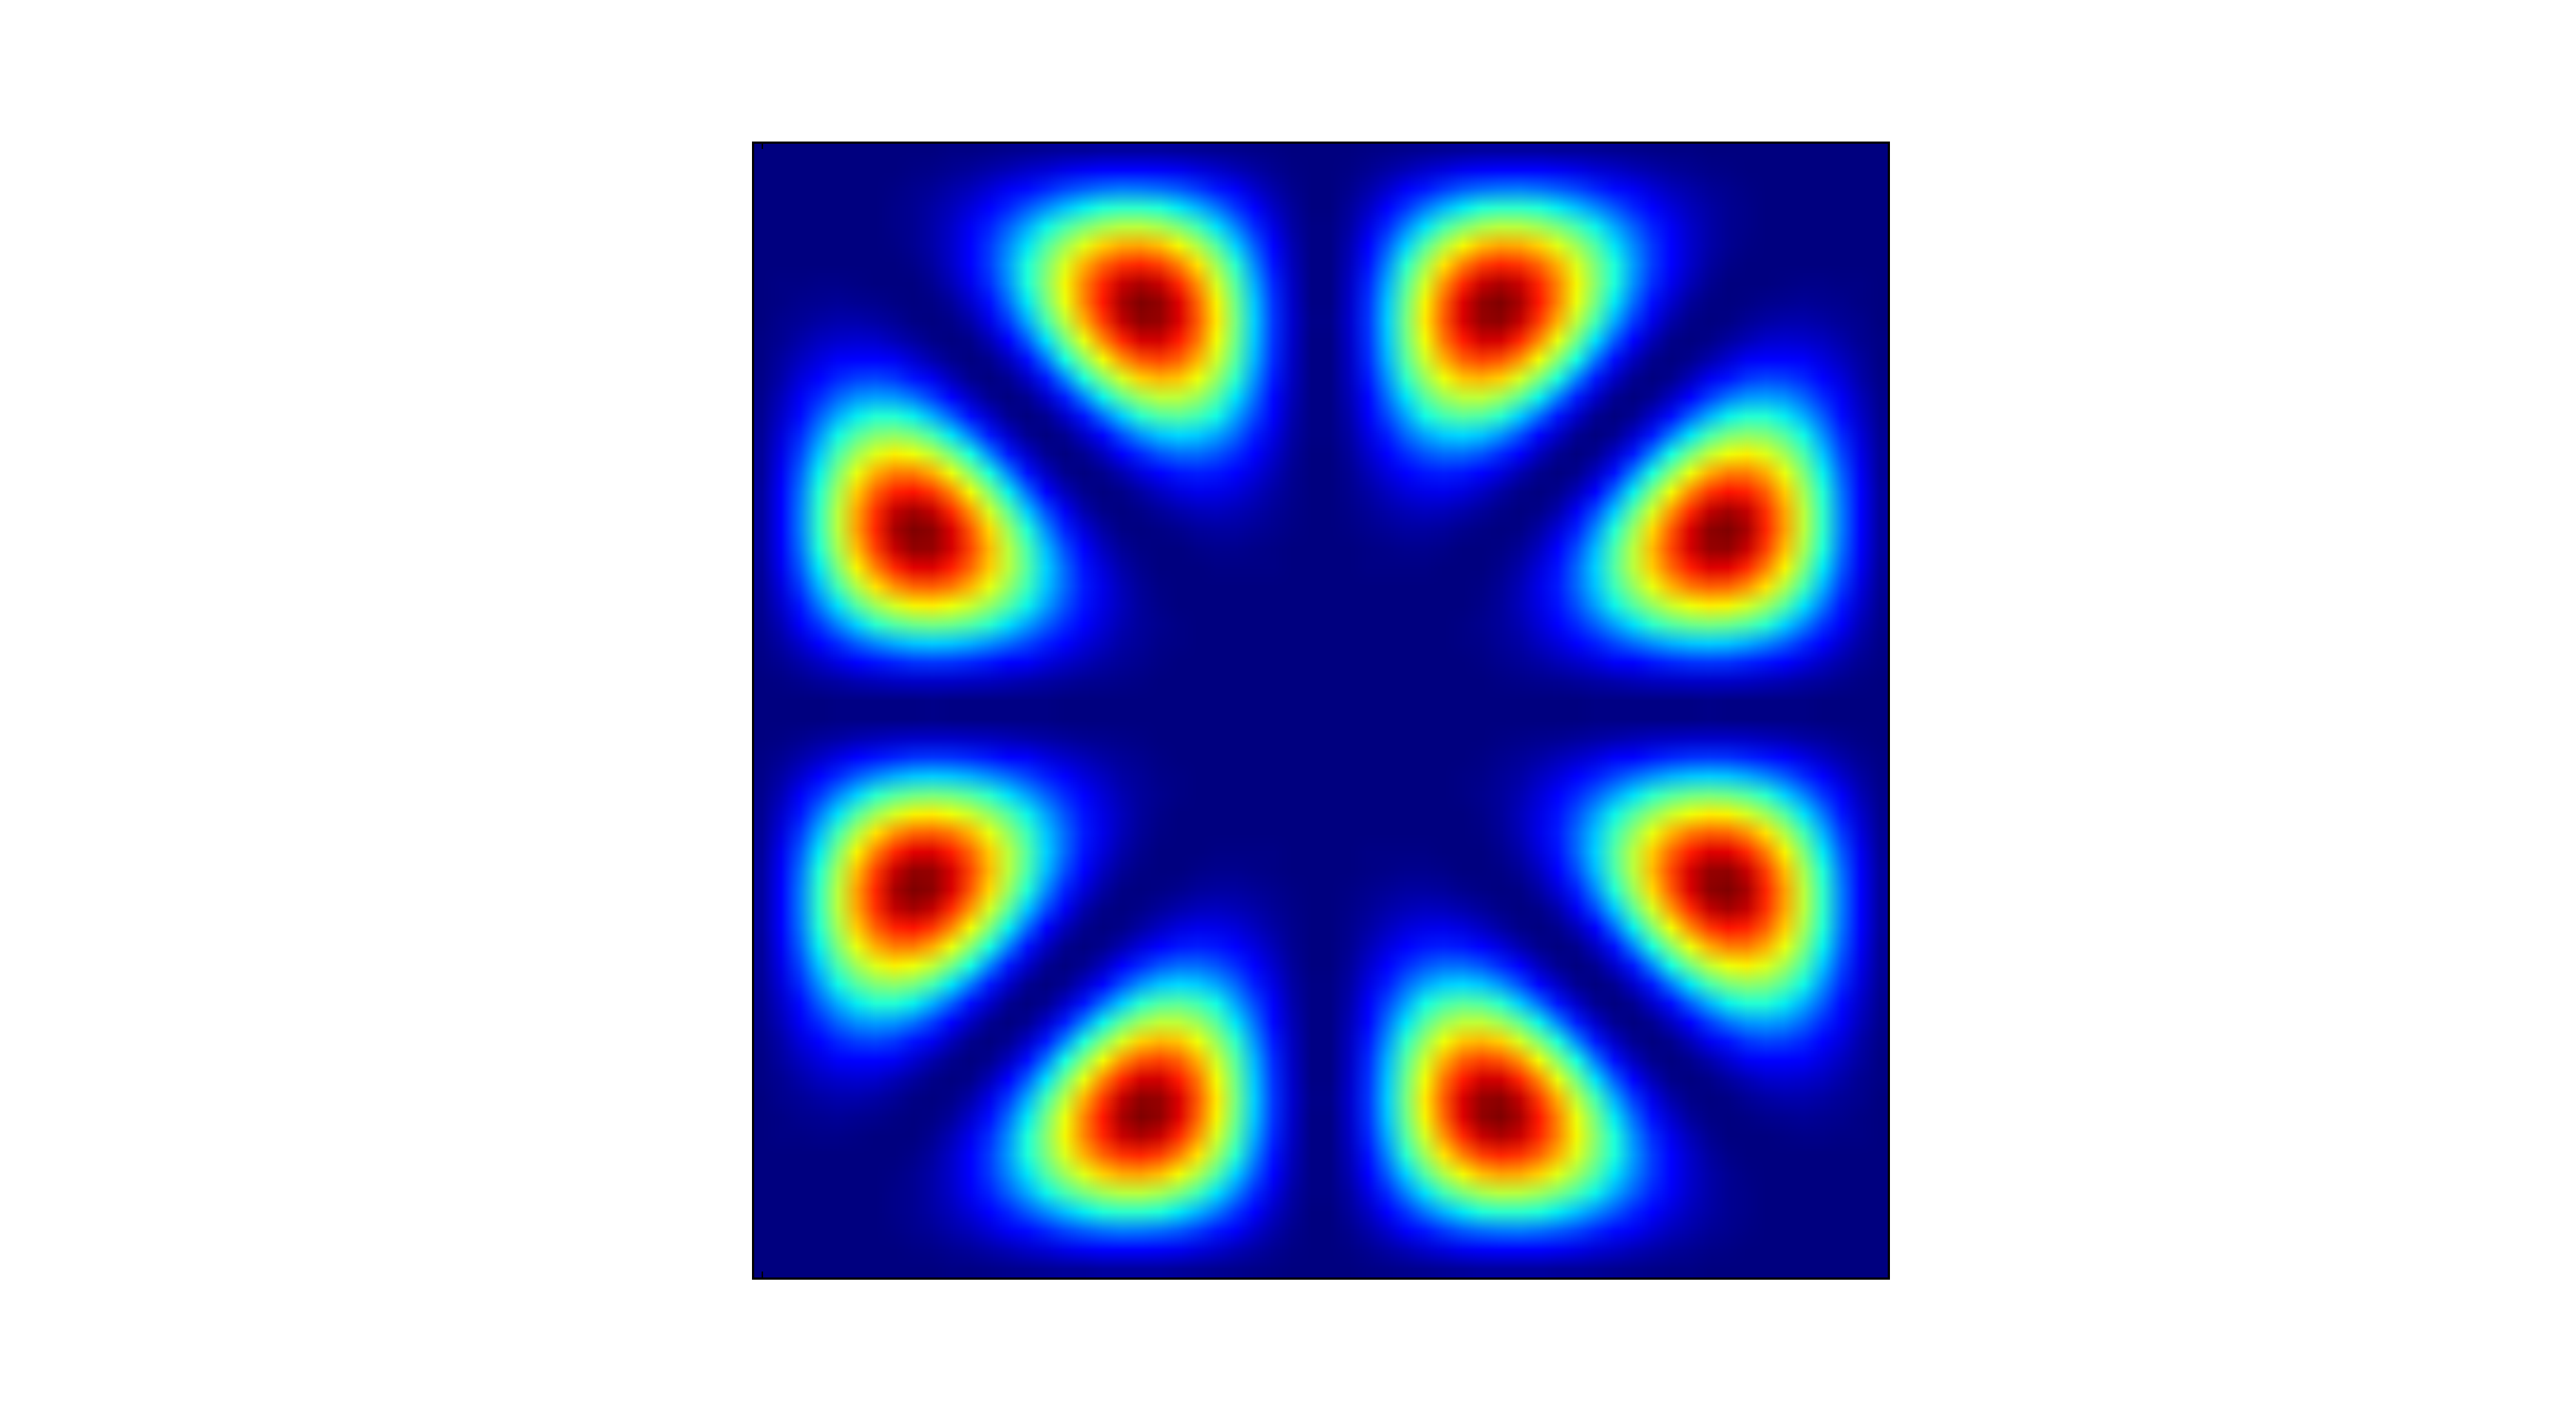
\includegraphics[width=\unitlength,page=1]{figures/2dn12.pdf}}%
    \put(0.29029359,0.02){\color[rgb]{0,0,0}\makebox(0,0)[lb]{\smash{$0$}}}%
    \put(0,0){\includegraphics[width=\unitlength,page=2]{figures/2dn12.pdf}}%
    \put(0.36680651,0.02){\color[rgb]{0,0,0}\makebox(0,0)[lb]{\smash{$0.17$}}}%
    \put(0.4426603,0.02){\color[rgb]{0,0,0}\makebox(0,0)[lb]{\smash{$0.33$}}}%
    \put(0.48651887,0.0524266){\color[rgb]{0,0,0}\makebox(0,0)[lb]{\smash{}}}%
    \put(0.51581787,0.02){\color[rgb]{0,0,0}\makebox(0,0)[lb]{\smash{$0.5$}}}%
    \put(0.58897543,0.02){\color[rgb]{0,0,0}\makebox(0,0)[lb]{\smash{$0.67$}}}%
    \put(0.66133219,0.02){\color[rgb]{0,0,0}\makebox(0,0)[lb]{\smash{$0.83$}}}%
    \put(0.7287978,0.02){\color[rgb]{0,0,0}\makebox(0,0)[lb]{\smash{$1$}}}%
    \put(0.25,0.11614262){\color[rgb]{0,0,0}\makebox(0,0)[lb]{\smash{$0.17$}}}%
    \put(0.25,0.19155608){\color[rgb]{0,0,0}\makebox(0,0)[lb]{\smash{$0.33$}}}%
    \put(00.25,0.2640038){\color[rgb]{0,0,0}\makebox(0,0)[lb]{\smash{$0.5$}}}%
    \put(0.25,0.33941722){\color[rgb]{0,0,0}\makebox(0,0)[lb]{\smash{$0.67$}}}%
    \put(00.25,0.41313597){\color[rgb]{0,0,0}\makebox(0,0)[lb]{\smash{$0.83$}}}%
    \put(0.25,0.48897306){\color[rgb]{0,0,0}\makebox(0,0)[lb]{\smash{$1$}}}%
    \put(0,0){\includegraphics[width=\unitlength,page=3]{figures/2dn12.pdf}}%
    \put(0.25,0.04920264){\color[rgb]{0,0,0}\makebox(0,0)[lb]{\smash{$0$}}}%
    \put(0.51560752,0){\color[rgb]{0,0,0}\makebox(0,0)[lb]{\smash{$x$}}}%
    \put(0.17751812,0.24572913){\color[rgb]{0,0,0}\makebox(0,0)[lb]{\smash{$y$}}}%
  \end{picture}%
\endgroup%
}
%	\caption{Propability densities for the calculated eigenfunction $\psi_{12}$, with the method of finite differences and a grid of $N=60$ in two dimensions. For simplicity the prefactor $\frac{\hbar^2}{2m}$ was set to one, obtaining a non-normalized eigenfunction.}
%\label{fig:2d_eigenfunction}
%\end{figure} 

In three dimensions, we obtain a $N^3$-dimensional Matrix, for example for $N=2$:
\begin{align*}
T \approx
\tiny
\begin{pmatrix}
 6 & -1 & -1 &  & -1 &  &  & \scalebox{3}{$0$}  \\\\
   -1 & 6 & -1 & -1 &  & -1 &  & \\\\
     -1 & -1 & 6 & -1 & -1 &  & -1 & \\\\
        & -1 & -1 & 6 & -1 & -1 &  & -1\\\\
        -1 &  & -1 & -1 & 6 & -1 & -1 & \\\\
           & -1 &  & -1 & -1 & 6 & -1 & -1\\\\
             &  & -1 &  & -1 & -1 & 6 & -1\\\\
              \scalebox{3}{$0$}  &  &  & -1 &  & -1 & -1 & 6\\\\
              \end{pmatrix}
\end{align*}

\begin{lstlisting}
Still Missing: Comparison with exact results
\end{lstlisting}

Referring back to the time expansion in chapter \ref{1}, the time evolution of an eigenfunction of the hamiltonian is trivial, since $\psi_t$ only differs in phase from the initial state $\psi_0$, so ${|\psi_t|}^2$ is time-independent, although linear combinations of eigenfunctions depend on time, which will not be calculated here.\\

If we take the computing time into account, it is obvious that even with a small grid size $N<100$ and parallelized computing the simulation of a particle in a square well potential lead to a unexecutable applications. The increase of dimensions with constant gridsize results in a growing computing time higher than $\mathcal O (t_0^n)$. \\

To proceed to coupled quantum mechanical systems it seems to be mandatory to use efficient approximations.




    \section{Many-Body Simulations}
    
    Consider a real physical system, where particles are not independent like in atoms, ions, molecules, etc. . Assuming the system consists only of $K$ nuclei and $N$ electrons the hamiltonian consists of the terms
\begin{align*}
    H = T_i + T_n+ V_{ii} + V_{in} + V_{nn} \text{ ,}
\end{align*} 
    where $T_i $ and $T_n$ are the kinetic energies of the electrons and nuclei, respectively. $V_{ii}$ represents the Coulomb repulsion between electrons, $V_{nn}$ between the nuclei and $V_{in}$  the attraction between electrons and nuclei. So the hamiltonian reads
    
    \begin{align*}
    H &= \sum_{i=1}^N \frac{p_i^2}{2m} + \sum_{n=1}^K \frac{P_n^2}{2M_n} + \frac{1}{4\pi \epsilon_0}\frac{1}{2}\sum_{i,j\neq 1, i \neq j}^N \frac{e^2}{|\mathbf{r}_i - \mathbf{r}_j|} \\ &-  \frac{1}{4\pi \epsilon_0}\sum_{i=1}^K \sum_{i=1}^N \frac{Z_n e^2}{|\mathbf{r}_j-\mathbf{R}_n|} +  \frac{1}{4\pi \epsilon_0}\frac{1}{2} \sum_{n,n'=1;n\neq n'}^K \frac{Z_n Z_{n'} e^2}{|\mathbf{R}_n - \mathbf{R}_{n'}|} \text{,}
    \end{align*} where $m$ is the electron mass and $M_n$ the nuclei mass. The index $i$ refers to the electrons, the index $n$ to the nuclei.
This hamiltonian describing the system looks quite complicated and in fact, computing the dynamics of this system seems to be unsolvable even for a few particles and an efficient super computer. Therefore, approximations must be made, still comprising the important information about the system. One approach is the Born-Oppenheimer approximation. It uses the fact that the nuclei are much heavier than the electrons, so the motions of the nuclei are much faster compared to the electrons, justifying to neglect the coulomb repulsion between the nuclei and the kinetic energy of the nuclei, so the approximated hamiltonian becomes
\begin{align}\label{eq:H_BO}
H_\text{BO} = \sum_{i=1}^N \frac{p_i^2}{2m}  + \frac{1}{4\pi \epsilon_0}\frac{1}{2}\sum_{i,j = 1, i \neq j}^N \frac{e^2}{|\mathbf{r}_i - \mathbf{r}_j|} -  \frac{1}{4\pi \epsilon_0}\sum_{i=1}^K \sum_{i=1}^N \frac{Z_n e^2}{|\mathbf{r}_j-\mathbf{R}_n|}  \text{.}
\end{align}  
The positions of the nuclei can be varied to find the minimum of the total energy.
    \subsection{The Hartree-Fock Method and Equations}
 In equation (\ref{eq:H_BO}) the antisymmetry of the wave functions was not taken into account. Fock extended the so called \textit{Hartree equation} by taking antisymmetry into account. The derivation of the \textit{Hartree} and \textit{Hartree-Fock equations} will not be given here, since the main aim here is the implementation of the method. Therefore see e.g. \cite[p. 56-60]{Thijssen2007} and \cite[chapter 3]{Jensen2013}. The \textit{Fock operator} is in natural units given by
 \begin{align} \label{eq:hf}
 \mathcal{F}\psi_k = &\left[-\frac{1}{2} \nabla^2 
 - \sum_n \frac{Z_n}{|\mathbf{r}- \mathbf{R}_n|}\right]\psi_k(\mathbf{x}) + \nonumber
 \sum_{l=1}^N \int \text{d}x' |\psi_l(\mathbf{x}')|^2 \frac{1}{|\mathbf{r}-\mathbf{r}'|} \psi_k(\mathbf{x}) \\
&- \sum_{l=1}^N \int \text{d}x' \psi^*(\mathbf{x}')\frac{1}{|\mathbf{r}-\mathbf{r}'|} \psi_k(\mathbf{x}')\psi_l(\mathbf{x})\text{,}
 \end{align}
 satisfying the \textit{Hartree-Fock equation}
 \begin{align*}
 \mathcal{F} \psi_k = \epsilon_k \psi_k \text{.}
 \end{align*} The fourth term in equation (\ref{eq:hf}) is called the exchange term \cite[p. 55]{Thijssen2007} and is nonlocal since the operator is acting on $\psi_k$, but the value at the position $\mathbf{r}$ is determined by the value assumed by $\psi_k$ at all possible positions $\mathbf{r}'$. The eigenvalues $\epsilon_k$ of the Fock operator are related to the total energy by
 \begin{align*}
 E &= \frac{1}{2} \sum_k [\epsilon_k + \braket{\psi_k|h|\psi_k}] \text{, with}\\
 \braket{\psi_k|h|\psi_k} &= \int \text{d}^3\mathbf{x}\; \psi_k^*(\mathbf{x}) \left[-\frac{1}{2} \nabla^2 
 - \sum_n \frac{Z_n}{|\mathbf{r}- \mathbf{R}_n|}\right] \psi_k(\mathbf{x}) \text{.}
 \end{align*} It is obvious that the Fock operator in equation (\ref{eq:hf}) which acts on $\psi_k$ also depends on $\psi_k$ itself.
    
    
    
    
    \subsection{The Roothaan Equation}
    For molecules numerical basis sets are not efficient, so we use atom centered basis sets to describe the molecular orbital
    \begin{align}\label{eq:orbital}
    \psi_k(\vec{x}) = \sum_{p=1}^M C_{pk} \chi_p (\vec{x})\text{,}
    \end{align}
    with $k = 1,\dots, M$, where $M$ is the number of basis states.
    So the Hartree-Fock equation reads
    \begin{align*}
    \mathcal{F} (\vec{x})   \psi_k(\vec{x}) &= \epsilon_k    \psi_k(\vec{x})\text{.} \quad \text{Using Eq. (\ref{eq:orbital}) yields}\\
    \mathcal{F} (\vec{x})  \sum_{p=1}^M C_{pk} \chi_p (\vec{x}) &= \epsilon_k \sum_{p=1}^M C_{pk} \chi_p (\vec{x})\text{.}\\
    \end{align*}
    We can now multiply from the left by a specific basis function $\chi_\nu$. Integrating over the space yields
    \begin{align*}
     \sum_{p=1}^M C_{pk} \int \chi_\nu^*(\vec{x})  \mathcal{F} (\vec{x}) \chi_p(\vec{x})\text{d}^3 \vec{x} & =  \epsilon_k  \sum_{p=1}^M C_{pk} \int \chi_\nu^*(\vec{x}) \chi_p(\vec{x})\text{d}^3 \vec{x}   \text{.}
    \end{align*}
    This can be written in matrix notation of the Hartree-Fock equations, expressed in the atomic orbital basis:
    \begin{align*}
    \sum_{p=1}^M C_{pk} F_{\nu p}  &= \epsilon_k \sum_{p=1}^M C_{pk} S_{\nu p}\\
    \mathbf{F} \mathbf{C_k} &= \epsilon_k \mathbf{S} \mathbf{C_k} \; \text{,}
    \end{align*} which is called the \textit{Roothaan equation}.
    Since the Fock operator itself depends on $\mathbf{C_k}$ we have the problem of self consistency, because $\mathcal{F}$ has the solution already inside. The Self Consistent Field Method (SCF) uses the approach to solve the above equation iteratively, until the solution deviates only small from the next iteration.
    
    
    % bib stuff
    \nocite{*}
    \addtocontents{toc}{\protect\vspace{\beforebibskip}}
    \addcontentsline{toc}{section}{\refname}    
    \bibliographystyle{plain}
    \bibliography{Bibliography}
\end{document}


